\documentclass{article}

% if you need to pass options to natbib, use, e.g.:
%     \PassOptionsToPackage{numbers, compress}{natbib}
% before loading neurips_2021

% Silence warning about neurips package
\usepackage{silence}
\WarningFilter{latex}{You have requested package}

% ready for submission
%\usepackage{../neurips/neurips_2021}

% to compile a preprint version, e.g., for submission to arXiv, add add the
% [preprint] option:
\usepackage[preprint]{../neurips/neurips_2021}

% to compile a camera-ready version, add the [final] option, e.g.:
%\usepackage[final]{../neurips/neurips_2021}

% to avoid loading the natbib package, add option nonatbib:
%    \usepackage[nonatbib]{neurips_2021}

\usepackage[utf8]{inputenc} % allow utf-8 input
\usepackage[T1]{fontenc}    % use 8-bit T1 fonts
\usepackage{hyperref}       % hyperlinks
\usepackage{url}            % simple URL typesetting
\usepackage{booktabs}       % professional-quality tables
\usepackage{amsfonts}       % blackboard math symbols
\usepackage{nicefrac}       % compact symbols for 1/2, etc.
\usepackage{microtype}      % microtypography
\usepackage{xcolor}         % colors
\usepackage{amsmath}
\usepackage{graphicx}
\usepackage{algpseudocode,algorithm}

% Set bibliography style for natbib (called out by the nips style file)
\bibliographystyle{abbrvnat}

% argmax and argmin operators
\DeclareMathOperator*{\argmax}{argmax}
\DeclareMathOperator*{\argmin}{argmin}

% Force algorithmic to use small font
%\makeatletter
%\renewcommand{\ALG@beginalgorithmic}{\small}
%\makeatother

\title{ECE 239AS Project Final Report \\ A Brief Survey of Q-learning Methods}

% The \author macro works with any number of authors. There are two commands
% used to separate the names and addresses of multiple authors: \And and \AND.
%
% Using \And between authors leaves it to LaTeX to determine where to break the
% lines. Using \AND forces a line break at that point. So, if LaTeX puts 3 of 4
% authors names on the first line, and the last on the second line, try using
% \AND instead of \And before the third author name.

\author{%
    Ryan Chau \\
    \texttt{chau\_ryan@yahoo.com}\\
    \And
    My-Quan Hong \\
    \texttt{myquan@yahoo.com} \\
    % examples of more authors
    \And
    Nathan Kang \\
    \texttt{nkang@gseis.ucla.edu} \\
    \And
    Christopher Munoz \\
    \texttt{cmunozcortes@ucla.edu} \\
}

\begin{document}

\maketitle

\begin{abstract}
    Q-learning was one of the most important breakthroughs in reinforcement
    learning when it was first published by \cite{watkins1989learning}. Since
    then, several new algorithms have improved upon different aspects of
    Q-learning and have lead to state-of-the-art performance on various
    benchmarks. On this project, we describe three such improvements: Deep
    Q-learning, Double Deep Q-learning, and Dueling Deep Q-learning. We also
    evaluate their performance on selected Atari games and discuss the
    experimental results.
\end{abstract}

\section{Introduction}
Although Q-learning is one of the most popular reinforcement learning
algorithms, it is known to overestimate action values because of the included
maximization step. This issue extends to Deep Q-learning networks (DQN), which
combines Q-learning with a flexible deep neural network to approximate the
action-value function. The objective of this project is to evaluate and describe
Double Deep Q Networks (Double DQN), an algorithm first proposed in
\citet{van2016deep} to reduce overoptimistic action-value estimates in Deep Q
Networks (\cite{mnih2015human}). A discussion of another algorithm which
improves on Deep Q-learning, Dueling DQN, will also be included for a more
comprehensive survey of value-based reinforcement learning (RL) algorithms
(\cite{wang2016dueling}).

All three architectures, DQN, Double DQN, and Dueling DQN, are able to learn
policies directly from preprocessed pixels from video games and they all achieve
scores that surpass human-level performance on Atari 2600 games.  The survey
will include a comparison of the performance of all three algorithms on four
Atari games from the Arcade Learning Environment (ALE)
(\cite{bellemare2013arcade}).

\section{Algorithms}

\subsection{Deep Q Network}
DQN combines Q-learning with a multi-layered neural network, and uses a target
network and experience replay to achieve stable training. In typical neural
networks, the learning target changes frequently. However, an unstable learning
target hinders training and learning. DQN uses a target network to copy
parameters $\theta^-$ from the online network every $\tau$ steps to keep the
target parameters fixed.  Additionally, neural networks are prone to overfitting
current episodes. Experience replay solves this problem by storing experiences,
including state transitions, rewards, and actions, i.e. all the necessary data
to perform Q-learning, and creates mini-batches to update the neural network.

Despite the improvements introduced in the DQN algorithm, Q-learning is known to
produce overoptimistic value estimates. Overoptimistic value estimates are not
necessarily problematic, provided that all values are uniformly high and the
relative action ranking is preserved. However, \citet{van2016deep} demonstrated
that the DQN algorithm, which combines Q-learning with a neural network,
overestimates value estimates substantially in empirical evaulations of Atari
games from the Arcade Learning Environment. Additionally, \citet{van2016deep}
proved that these DQN overestimates are not uniform, and differ for different
states and actions.

Algorithm~\ref{alg:dqn} shows the complete pseudocode for Deep Q-learning. The
learning target is
\begin{equation}\label{eq:dqn}
    y_i^{\text{DQN}} = r + \gamma \max_{a'} \hat{Q}(s', a'; \theta^-)    
\end{equation}
where $\theta^-$ represents the parameters of the target network, and $\theta$
the parameters of the online network. The source of Q-learning and DQN's
optimistic tendencies is the learning target's max operator, which uses the same
values to both select and evaluate an action.

\begin{algorithm}[ht]
%\setstretch{1.25}
\caption{Deep Q-learning with experience replay}\label{alg:dqn}
\begin{algorithmic}[1]
    \State Initialize replay memory $\mathcal{D}$ to capacity $N$
    \State Initialize action-value function $Q$ with random weights $\theta$
    \State Initialize target action-value function $\smash{\hat{Q}}$ with
    weights $\theta^- = \theta$
    \For{episode $m \gets 1,\dots,M$}
        \State Observe initial frame $x_1$ and preprocess frame to get state
        $s_1$
        \For{time step $t \gets 1,\dots,T$}
            \State With probability $\varepsilon$ select a random action $a_t$;
            otherwise select $a_t = \argmax_a Q(s_t, a; \theta)$
            \State Execute action $a_t$ in emulator and observe reward $r_t$ and
            image $x_{t+1}$
            \State Preprocess $s_t$, $x_{t+1}$ to get $s_{t+1}$
            \State Store transition $(s_t, a_t, r_t, s_{t+1})$ in replay buffer
            $\mathcal{D}$
            \State Sample uniformly a random minibatch of $N$ transitions $(s_j,
            a_j, r_j, s_{j+1})$ from $\mathcal{D}$
            \State Set $y_j = r_j$ if episode ends at step $j+1$; \newline
                \hspace*{4em} otherwise set $\smash{y_j = r_j + \gamma \max_{a'}
                \hat{Q}(s_{j+1}, a'; \theta^-)}$
            \State Perform a stochastic gradient descent step on $J(\theta) =
            \tfrac{1}{N} \sum_{j=1}^{N} (y_j - Q(s_j, a_j; \theta))^2$ \newline
                \hspace*{4em} with respect to parameters $\theta$
            \State Every $c$ steps reset $\smash{\hat{Q} = Q}$
        \EndFor
    \EndFor
\end{algorithmic}
\end{algorithm}

\subsection{Double Deep Q Network}
Double Q-learning, which was proposed to alleviate the overestimation issue in
Q-learning, was subsequently shown to be effective in solving the weaknesses of
DQN and producing state-of-the-art results.  Double DQN combines Double
Q-learning with a neural network and produces more accurate value estimates and
better policies than DQN.  The $\max$ operator in \eqref{eq:dqn} uses the same
network to select and to evaluate an action, which \cite{van2016deep}
demonstrated leads to overestimates of the action values. To reduce
overestimations, \cite{hasselt2010double} showed that action selection and
action evaluation can be decoupled when computing the learning target in the
original Q-learning algorithm. \cite{van2016deep} showed that the same idea can
be applied to DQN to produce a new learning target,
\begin{equation}
    y_i^{\text{DoubleDQN}} = r + \gamma \hat{Q}(s', \argmax_{a'}
    \hat{Q}(s',a';\theta_i) \theta^-)
\end{equation}
Greedy action selection is now done according to the online network with
parameters $\theta$, but the value is estimated by the target network with
parameters $\theta^-$.  This simple, yet effective, modification to DQN is known
as Double DQN (or DDQN). 

\subsection{Dueling DQN}
The dueling network architecture by \cite{wang2016dueling} takes into account
the observation that for many states, it is unnecessary to estimate the value of
each action at every timestep. Dueling DQN utilizes the convolutional layers in
DQN and DDQN, but splits the network into two different streams: one for the
estimation of state-values and one for estimation of advantages for each action.
This introduces the advantage function, which estimates how advantageous it is
to select an action compared to others at the same state. This function takes
takes into account the state-value and Q functions.
\begin{equation}
    A^{\pi}(s, a) = Q^{\pi}(s,a) - V^{\pi}(s)
\end{equation}

Dueling DQN has a shortcoming in that the state-values and advantage function
are not uniquely recoverable given Q alone. To address this problem,
\cite{wang2016dueling} implement the following forward mapping for the final
set of Q values:
\begin{equation}
    Q(s,a; \theta, \beta)  = V(s; \theta, \beta) + (A(s, a; \theta, \alpha) - 
    \max_{a' \epsilon \vert \mathcal{A} \vert} A(s, a; \theta, \alpha))
\end{equation}

Algorithm~\ref{alg:double} shows the complete pseudocode for Dueling DQN.
The learning target for Dueling DQN is:
\begin{equation}
    y_i^{\text{DuelingDQN}} = r + \gamma \mathbb{E}_{a' \sim \pi (s') }
    [Q(s', a'; \theta_{i})]
\end{equation}


%Dueling DQN algorithm
\begin{algorithm}[ht]
%\setstretch{1.25}
\caption{Double DQN with Dueling network}\label{alg:double}
\begin{algorithmic}[1]
    \State Initialize empty replay buffer $\mathcal{D}$ to capacity $N$
    \State Initialize $\theta$ - initial network parameters, $\theta^{-}$ - copy
    of $\theta$

    \For{episode $m \gets 1,\dots,M$}
        \State Initialize frame sequence $x \gets ()$ 
        \For{time step $t \gets 1,\dots,T$}
            \State Set state $s \gets x$, sample action $a \sim
            \pi_{\mathbb{B}}$
            \State Sample next frame $x^{t}$ from environment
            $\mathbf{\varepsilon}$
            given $(s,a)$ and receive reward $r$, and append \newline
                \hspace*{4em} $x^{t}$ to $x$
            \If{$\vert x \vert > N_{f}$}
                \State delete oldest frame $x_{t_{\min}}$ from $x$
            \EndIf
            \State Set $s' \gets x$, and add transition tuple $(s, a, r, s')$ to
            $\mathcal{D}$, replacing the oldest tuple if $\mathcal{D} \geq
            N_{r}$
            \State Sample a  minibatch of $N_{b}$ tuples $(s, a, r, s') \sim$
            Unif$(\mathcal{D})$
            \State Construct target values, one for each of the $N_{b}$ tuples:
            \State Define $a^{\max}(s';\theta) = \argmax_{a'}Q(s', a'; \theta)$
            \State Define $Q(s', a'; \theta)=V(s; \theta) + (A(s', a'; \theta)
            - \max_{a' \epsilon \vert \mathcal{A} \vert} A(s, a'; \theta))$
            \State Set $y_{j} = r$ if s' is terminal; otherwise set
            $\smash{y_{j} = r + \gamma Q(s', a^{\max}(s';\theta); \theta^{-})}$
            \State Perform a gradient descent step with loss $\vert \vert y_j -
            Q(s_j, a_j; \theta) \vert \vert ^2$ 
            \State Replace target parameters $\theta^{-} \gets \theta$ every
            $N^{-}$ steps 
        \EndFor
    \EndFor
\end{algorithmic}
\end{algorithm}


\section{Experimental Results}
To conduct an evaluation of the performance of the algorhtms we used an
implementation based on the Tensorpack framework (\cite{wu2016tensorpack}).
Tensorpack is an interface built on TensorFlow v1 that is focused on training
speed. Its low overhead and support for training with a GPU provided us with a
way to train the models from scratch in Google Colab Pro instances, within a
reasonable amount of time (roughly 24 hours for each Atari game). 

Each model was trained for 5 million training steps (200 epochs) on the
following games from the Atari Learning Environment (ALE)
(\cite{bellemare2013arcade}): \texttt{Breakout-v0}, \texttt{RoadRunner-v0},
\texttt{Boxing-v0}, and \texttt{VideoPinball-v0}. Note that Dueling DQN run of
video pinball was trained for roughly 170 epochs due to Google Colaboratory GPU
usage limits. After training, the models were evaluated over 100 episodes in
order to get mean scores for each game. The scores were normalized based on
recorded human scores and random scores as follows:

\begin{equation}
    \text{score}_\text{normalized} = \frac{\text{score}_\text{agent} 
        - \text{score}_\text{random}}
        {\text{score}_\text{human} - \text{score}_\text{random}}
\end{equation}

The random and human scores presented in Table \ref{tab:models} are the same 
as those used by \cite{mnih2015human} and \cite{van2016deep}.

\begin{table}[ht]
\centering
\small
\begin{tabular}{lcc} 
\toprule
\multicolumn{1}{c}{Game} & 
\begin{tabular}[c]{@{}c@{}}Random\end{tabular} & 
\begin{tabular}[c]{@{}c@{}}Human\end{tabular} \\ 
\hline \hline
Boxing & 0.10 & 4.30   \\
Breakout & 1.70 & 31.80  \\
Road Runner & 11.50 & 7845.00   \\
Video Pinball & 16256.90 & 17297.60   \\
\bottomrule
\end{tabular}
\caption{Random and Human Scores for Normalization}
\label{tab:models}
\end{table}

Figure \ref{fig:training} shows the mean scores achieved by each model during
training on each of the four selected Atari games. Figure \ref{fig:eval} shows
the normalized scores achieved by each model during evaluation on each of the
four selected Atari games.

\begin{figure}[ht]
    \centering
    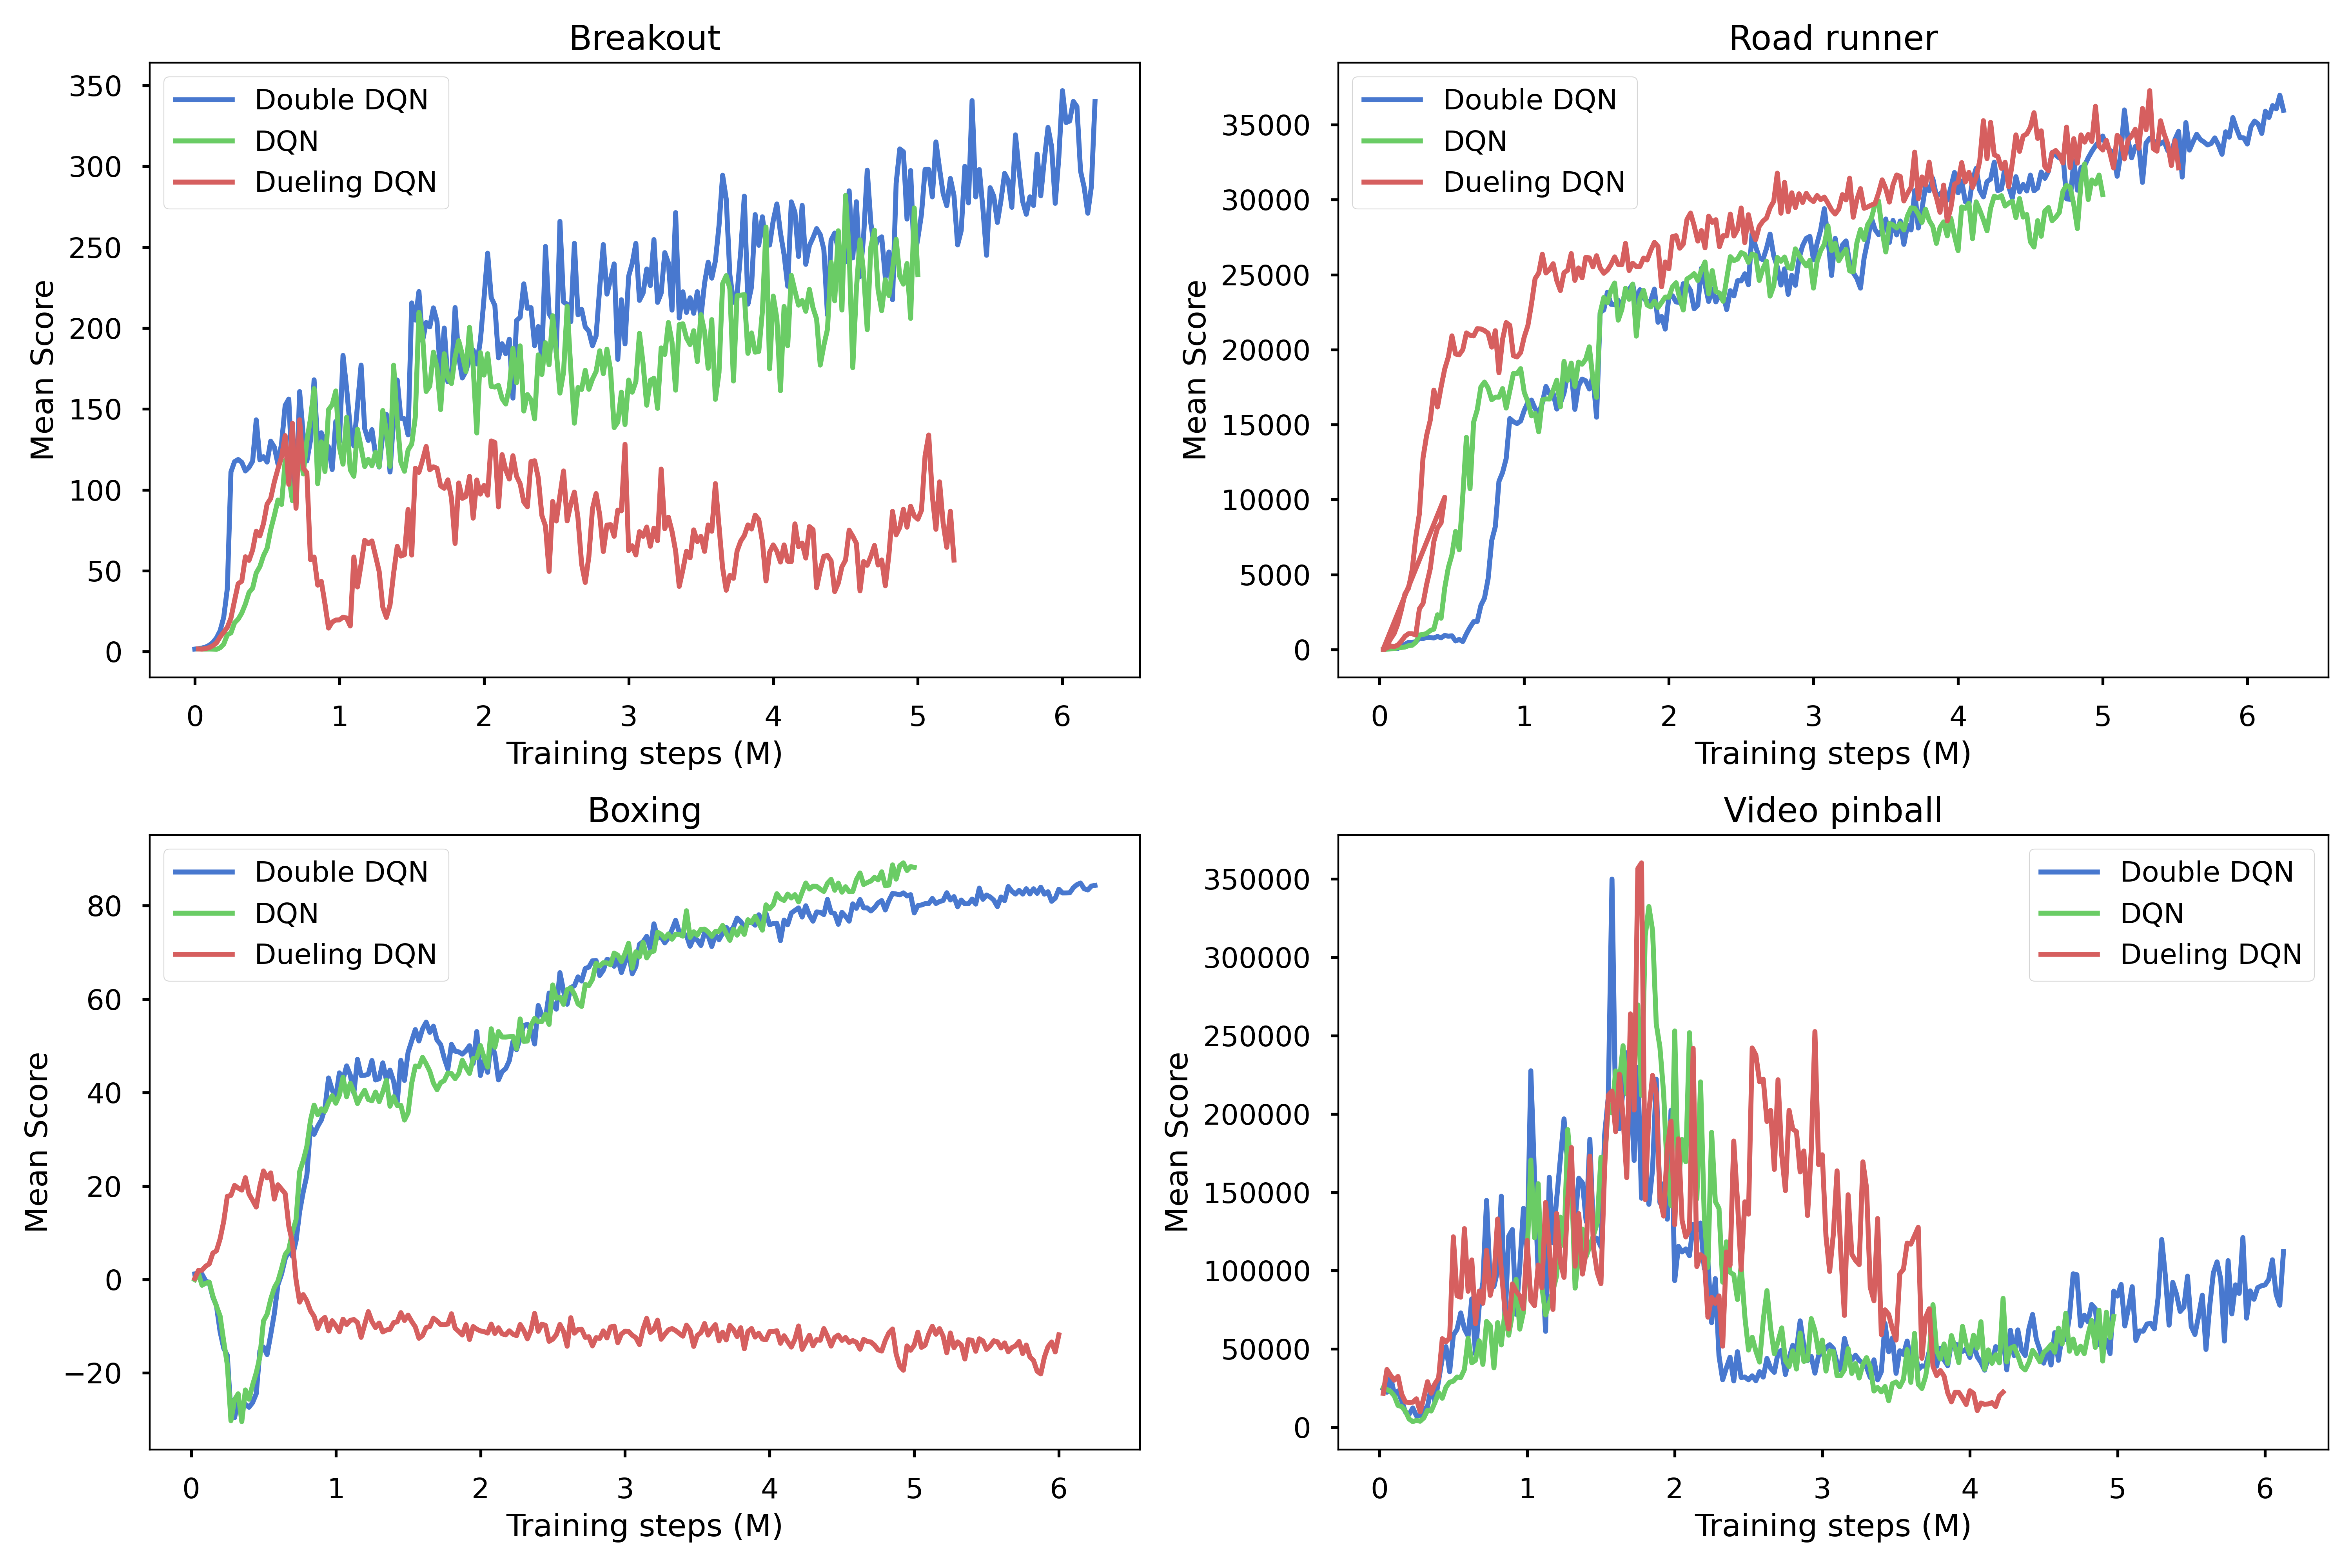
\includegraphics[width=\linewidth]{double_dqn-mean_scores.png}
    \caption{Mean score over training steps for selected games from the Atari
    Learning Environment (ALE).}
    \label{fig:training}
\end{figure}

\begin{figure}[ht]
    \centering
    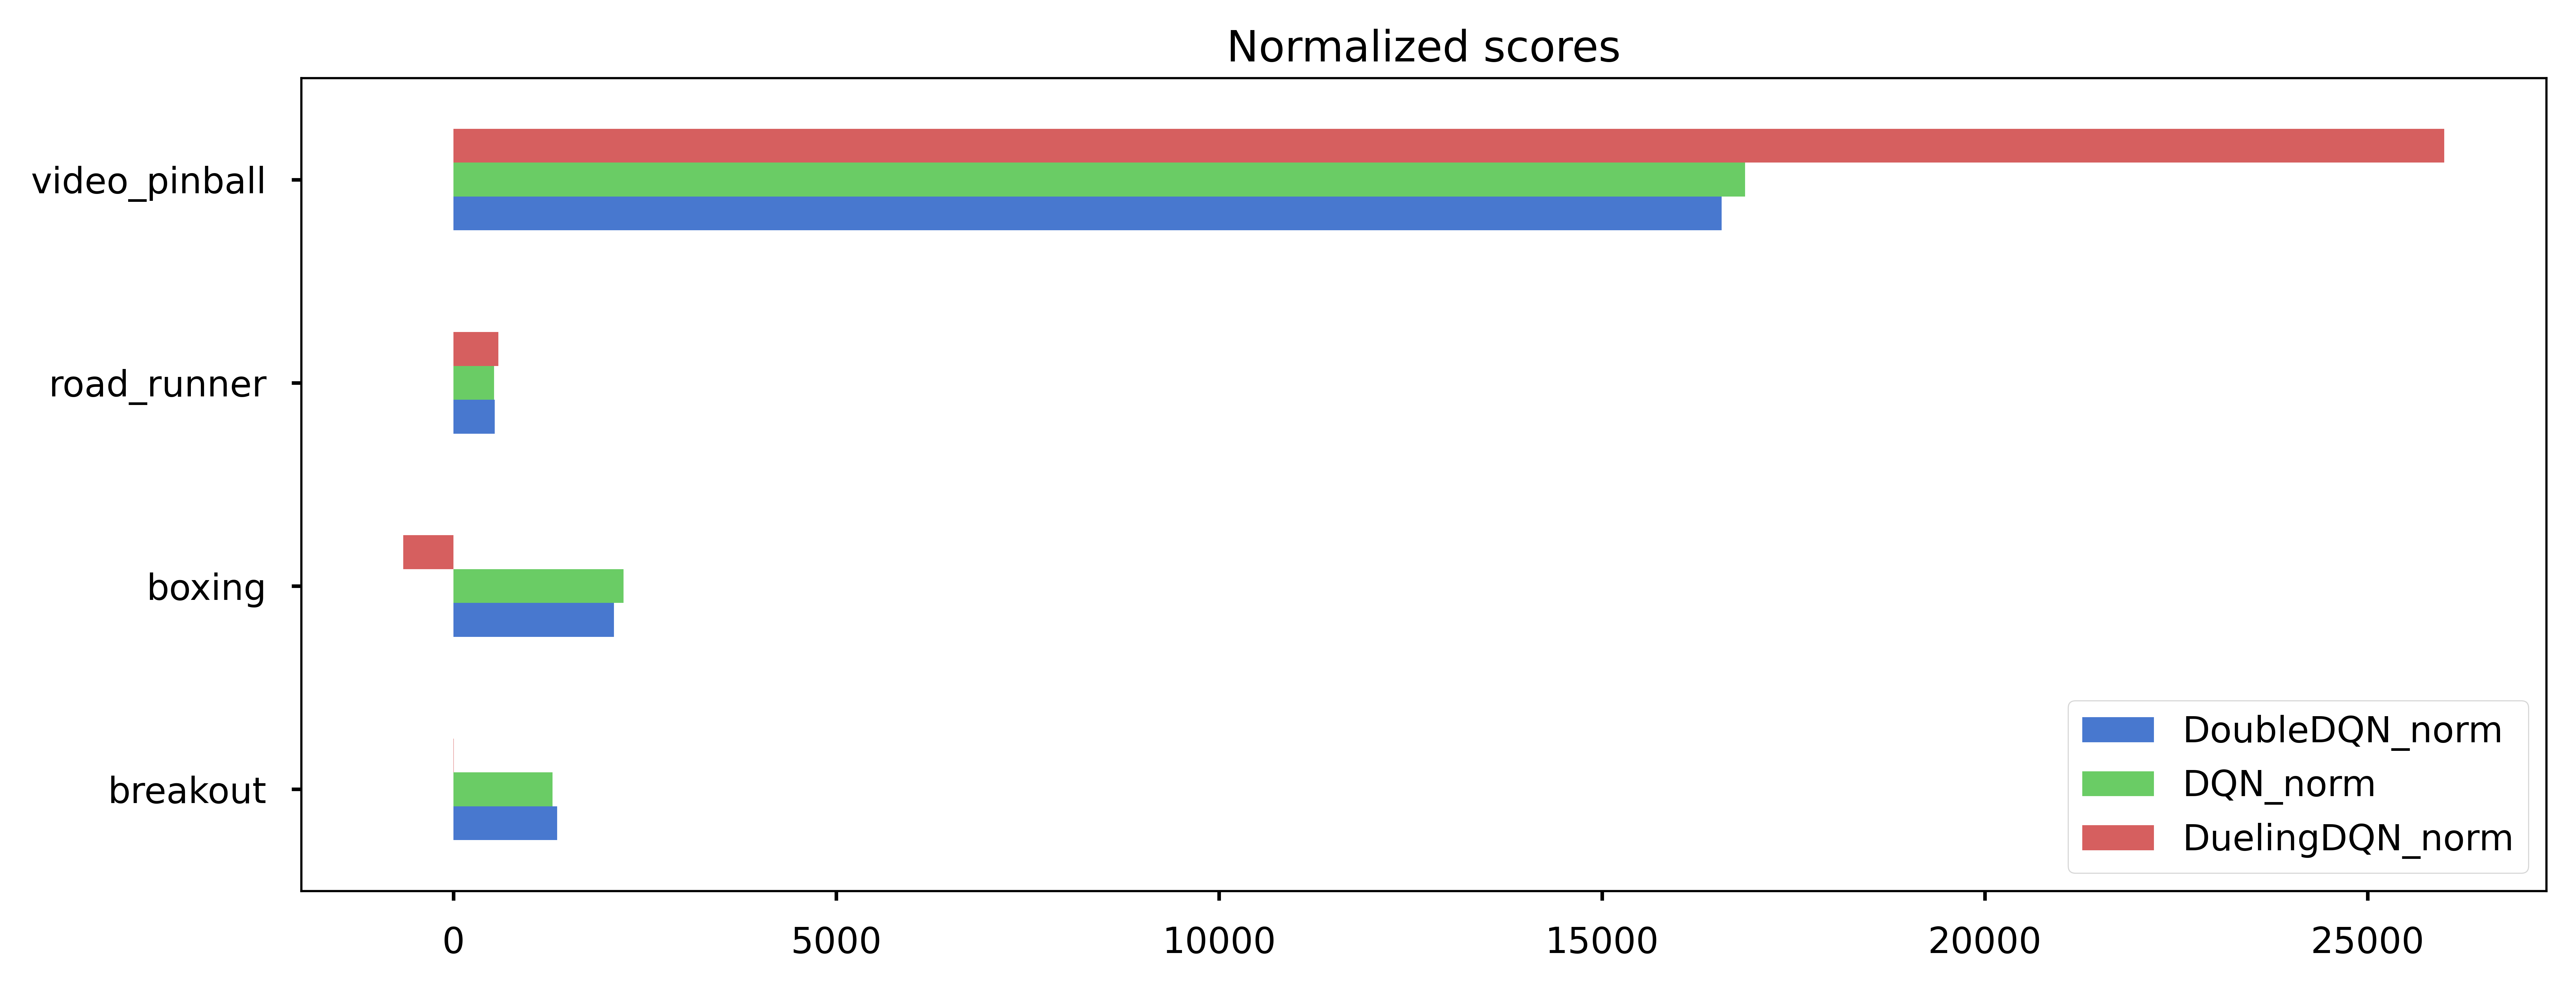
\includegraphics[width=\linewidth]{norm_scores.png}
    \caption{Normalized evaluation score over 100 episodes for selected games
    from the Atari Learning Environment (ALE).}
    \label{fig:eval}
\end{figure}

The mean scores achieved by DQN, Double DQN, and Dueling DQN during training
were comparable on Road Runner, although Double DQN and Dueling DQN's mean
scores are slightly higher than DQN.  Additionally, DQN and Double DQN produced
comparable mean score results on Bowling. However, Double DQN performed better
than DQN on  Breakout and Video Pinball, demonstrating the negative effects of
DQN's overestimations.  

Although Dueling DQN can produce dramatic improvements over DQN and Double DQN,
this was not empirically observed in the Dueling DQN scores for Breakout and
Boxing. The Dueling DQN mean scores for Boxing and Breakout were significantly
lower than DQN and DDQN, and produced equally poor evaluation results.  However,
this poor performance is in alignment with the Atari empirical study results
presented in \cite{wang2016dueling}. In their paper, \cite{wang2016dueling}
showed that the Dueling DQN normalized score was only 3.46\% better than Double
DQN for Boxing, and 17.56\% worse than Double DQN for Breakout. It is possible
that Dueling DQN was not trained long enough to demonstrate performance
enhancements over DQN and Dueling DQN.

In terms of model evaluation normalized scores, DQN performed the best in
Boxing, Double DQN performed best in Breakout, and Dueling DQN performed best in
Road Runner and Video Pinball. Evaulation results were low for Dueling DQN in
Breakout and Boxing, which aligns with the mean training scores.

\section{Conclusion}
Deep Q-learning methods are some of the core algorithms in Reinforcement
Learning and they are behind some of the most important breakthroughs in the
field. Deep Q Networks, developed by DeepMind in 2015, reached (and in many
cases surpassed) human-level performance across a variety of Atari games. DQN
combined the classical Q-learning algorithm developed by
\cite{watkins1989learning} with deep neural networks, and a technique known as
\emph{experience replay}. DQN, however, suffered from the same issue as
Q-learning, namely overestimation of the action values due to the max operator
used in action selection and evaluation. Double Q-learning, which reduced
overoptimistic value estimation in standard Q-learning, was also shown to be an
effective proposition in DQN. The algorithm, which came to be known as Double
DQN, effectively used two networks to decouple action selection and action
evaluation. Evaluation of the algorithm on games from the Atari Learning
Environment showed that reducing overestimation of action values with Double DQN
considerably improved performance on several games and led to better policies
than DQN. In that sense, we were sucessful in replicating these results; we
observed better scores for Double DQN in three out of the four games, and worse
results in one of the four games, though the latter was expected based on the
results reported in \cite{van2016deep}.

Dueling DQN, developed by \cite{wang2016dueling}, represents another improvement
over DQN. Motivated by the fact that in many states the choice of action is
inconsequential, Dueling DQN splits the single stream of fully connected layers
into two: one to estimate the state-value function and the other to estimate the
advantage function. Both estimates are combined at the last layer into a single
Q-function. Now, since Dueling DQN shares the same input-output relationship as
DQN and Double DQN, all learning algorithms with Q networks (such as DQN and
Double DQN) can be used to train the dueling architecture. Our evaluation of the
Dueling DQN architecture on selected Atari games yielded results that generally
matched those reported by \cite{wang2016dueling} on the four games. In the game
of video pinball, we saw the highest performance increased for Dueling DQN over
DQN and DDQN. In boxing, our evaluation results did not quite match those from
\cite{wang2016dueling}; while the results from the latter were positive, but
worse than DQN and DDQN, ours were negative and much significantly worse than
DQN and DDQN. The likely reason for this discrepancy is that we only trained for
4-5 million training steps compared to 200 million as reported on the references
papers.

% Import bibliography from ref.bib
\bibliography{ref}

\end{document}
